%%%%%%%%%%%%%%%%%%%%%%%%%%%%%%%%%%%%%%%%%
% University Assignment Title Page 
% LaTeX Template
% Version 1.0 (27/12/12)
%
% This template has been downloaded from:
% http://www.LaTeXTemplates.com
%
% Original author:
% WikiBooks (http://en.wikibooks.org/wiki/LaTeX/Title_Creation)
%
% License:
% CC BY-NC-SA 3.0 (http://creativecommons.org/licenses/by-nc-sa/3.0/)
% 
% Instructions for using this template:
% This title page is capable of being compiled as is. This is not useful for 
% including it in another document. To do this, you have two options: 
%
% 1) Copy/paste everything between \begin{document} and \end{document} 
% starting at \begin{titlepage} and paste this into another LaTeX file where you 
% want your title page.
% OR
% 2) Remove everything outside the \begin{titlepage} and \end{titlepage} and 
% move this file to the same directory as the LaTeX file you wish to add it to. 
% Then add \input{./title_page_1.tex} to your LaTeX file where you want your
% title page.
%
%%%%%%%%%%%%%%%%%%%%%%%%%%%%%%%%%%%%%%%%%
%\title{Title page with logo}
%----------------------------------------------------------------------------------------
%	PACKAGES AND OTHER DOCUMENT CONFIGURATIONS
%----------------------------------------------------------------------------------------

\documentclass[12pt]{article}
\usepackage[english]{babel}
\usepackage[utf8x]{inputenc}
\usepackage{amsmath}
\usepackage{graphicx}
\usepackage[colorinlistoftodos]{todonotes}
\usepackage{setspace}
\usepackage{hyperref}

\begin{document}
	
	\begin{titlepage}
		
		\newcommand{\HRule}{\rule{\linewidth}{0.5mm}} % Defines a new command for the horizontal lines, change thickness here
		
		\center % Center everything on the page
		
		%----------------------------------------------------------------------------------------
		%	HEADING SECTIONS
		%----------------------------------------------------------------------------------------
		
		\textsc{\LARGE University of Lille 1}\\[1.5cm] % Name of your university/college
		%\textsc{\Large Major Heading}\\[0.5cm] % Major heading such as course name
		%\textsc{\large Minor Heading}\\[0.5cm] % Minor heading such as course title
		
		%----------------------------------------------------------------------------------------
		%	TITLE SECTION
		%----------------------------------------------------------------------------------------
		
		\HRule \\[0.4cm]
		\huge \bfseries Privacy-preserving Data Dissemination in Mobile Crowd-Sensing\\[0.4cm] % Title of your document
		\HRule \\[1.5cm]
		
		%----------------------------------------------------------------------------------------
		%	AUTHOR SECTION
		%----------------------------------------------------------------------------------------
		
		\begin{minipage}{0.4\textwidth}
			\begin{flushleft} \large
				\emph{Author:}\\
				Romain \textsc{Sommerard} % Your name
			\end{flushleft}
		\end{minipage}
		~
		\begin{minipage}{0.4\textwidth}
			\begin{flushright} \large
				\emph{Supervisor:} \\
				Romain \textsc{Rouvoy} % Supervisor's Name
			\end{flushright}
		\end{minipage}\\[2cm]
		
		% If you don't want a supervisor, uncomment the two lines below and remove the section above
		%\Large \emph{Author:}\\
		%John \textsc{Smith}\\[3cm] % Your name
		
		%----------------------------------------------------------------------------------------
		%	DATE SECTION
		%----------------------------------------------------------------------------------------
		
		{\large \today}\\[2cm] % Date, change the \today to a set date if you want to be precise
		
		%----------------------------------------------------------------------------------------
		%	LOGO SECTION
		%----------------------------------------------------------------------------------------
		
		
\includegraphics[width=0.5\textwidth]{images/logo.png}\\[1cm] % Include a department/university logo - this will require the graphicx package
		
		%----------------------------------------------------------------------------------------
		
		\vfill % Fill the rest of the page with whitespace
		
	\end{titlepage}
	
	
	%\begin{abstract}
	%	Your abstract.
	%\end{abstract}
	
	\newpage
	
	\tableofcontents
	
	\newpage
	
	\section{Introduction}
	\label{sec:intoduction}
	
%%%% OK

Our two contributions for crowd-sensing platforms are as follows:
\begin{itemize}
	\item Foug\`ere, a data dissemination library that uses a distance notion to disseminate data.
	The library comes with 3 defaults dissemination modules: Wi-Fi Direct, Social and Contextual.
	\item AndroFleet, a large-scale emulation platform that includes a WiFi-Direct emulation implementation for the Android platform. 
	This emulation platform is a tool that permits the testing of crowd-sensing applications in the context of a crowd of devices. 
	AndroFleet trends to be as near as possible to the real usage of the application on real mobile devices.
\end{itemize}

The reminder of this paper is structured as follows. In Section \ref{sec:context_motivation} we introduce the context and motivations that remain to this work. Section \ref{sec:contribution} presents the principles used by the Foug\`ere library. Section \ref{sec:implementation_details} describes important points of Foug\`ere. Then, in the Section \ref{sec:evaluation} we present AndroFleet and the results of the contribution. Finally, in Section \ref{sec:conclusion_perspectives} we summarize and discuss future possible works.

%%%% END OK
	
	\section{Context \& Motivations}
	\label{sec:context_motivation}
	
%%%% OK

In this section we discuss the context underlining our contribution and present the motivations that led to our approach.

\subsection{Context: Mobile Crowd-Sensing Platforms}

The crowd-sensing platforms have a large application domain.
The applications encompass application performance monitoring (\emph{e.g.}, OpenSignal\footnote{\url{http://opensignal.com}}), environment monitoring (air quality\footnote{\url{http://citizensensor.cc}}), etc.
\\

Privacy-preserving in this context is a key challenge to address.
The platforms must balance to find an equilibrium between the level of the users' privacy-preserving and the quality of the data that are collected.
Indeed, if a crowd-sensing platform put a lot of consideration in the privacy preserving, the collected data could be degraded depending to the data type.
At last, if a crowd-sensing platform does not care about the privacy of its users, the latter may not want to contribute to it.
To the best of our knowledge, privacy-preserving techniques are often deployed on the server side~\cite{DBLP:conf/mobisys/CorneliusKKPST08}~\cite{DBLP:conf/dais/HadererRS13}.
For instance, for the Geo-located data, there can be anonymized \emph{a posteriori}~\cite{DBLP:conf/icdcs/PrimaultMB15}.
\\

The context to this proposal is based on the APISENSE crowd-sensing platform that provide an Android application to collect data from users.
Those users subscribe to data collect campaign and contribute with their mobile devices.
Because the platform applies privacy-preserving techniques on the server side, it does not protect from malicious behaviors during the upload phase.
The data coming from a user are unmodified and are his own data.
Those data were produced by this specific user.
A user is, therefore, forced to trust the server that receives his data.

\subsection{Motivations: Data Dissemination Threats}

In the APISENSE platform, a collect server, also called Honeycomb, can be managed by an external organization.
\\

Having multiple servers is a requirement because a single server cannot handle all users' data that are sent during a collect campaign.
Moreover, for the users' privacy, no server can be trusted.
\\

A key challenge in the crowd-sensing platforms is to avoid central trusted server that present a single point of failure that need to be addressed.

\begin{figure*}[h]
    \centering
    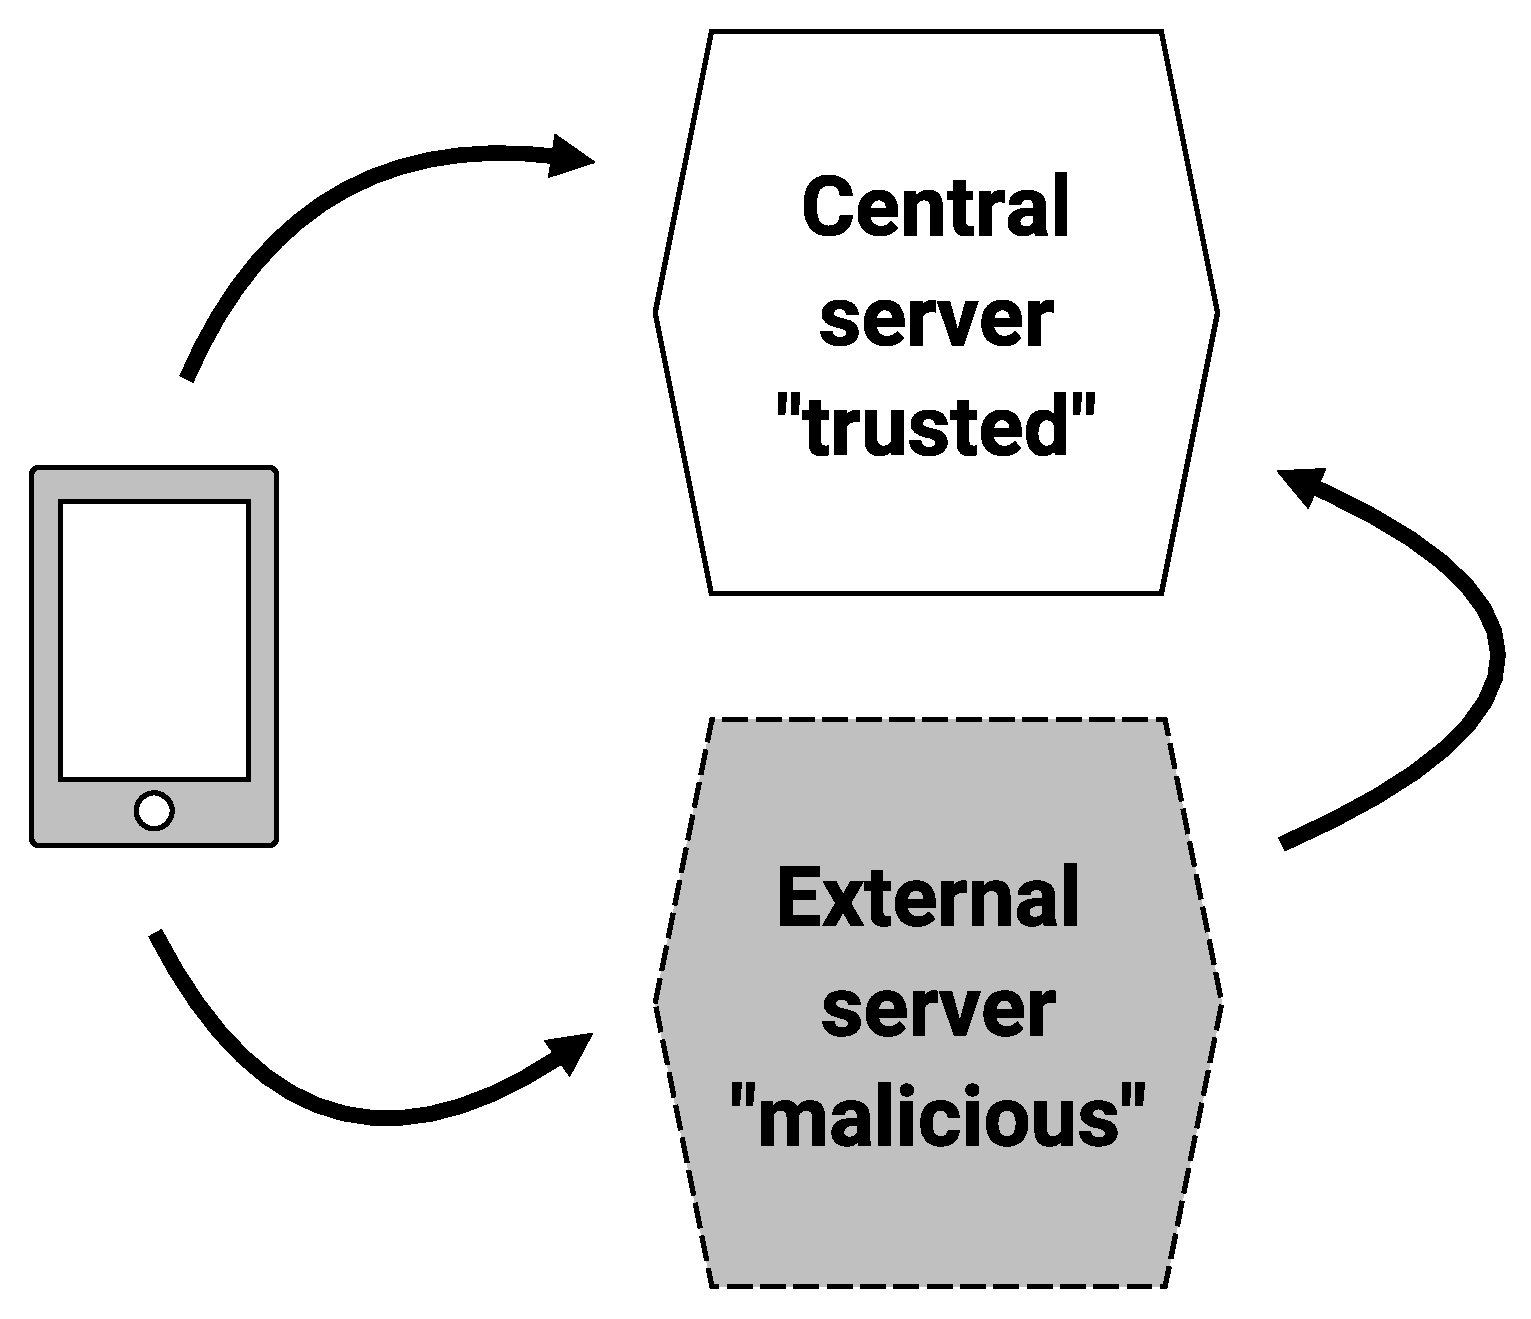
\includegraphics[width=0.5\textwidth]{figures/threat}
    \caption{\label{Threat} APISENSE data collection threat}
\end{figure*}

The current process of data collection is represented in Figure~\ref{Threat}.
\\

Let assume a user that participates to a data collect campaign.
Currently, the user produces data and sends it directly to a collect server.
The user has no control on the server selection that will receive the data.
The server that receives the data knows irremediably that those data are produced by the user that sends it.
The server that collects the data can be a trusted server or, as exposed before, an external server managed by an organization that can be potentially malicious.
The threat on a malicious server is that it can use the data against the user and deduct privacy information about it.
Furthermore, even if the data are collected by a trusted collect server, the threat can come from a malicious person that listen the transmission channels or steals the data stored on the server.
This kind of threats is not viable for privacy concerns.
\\

To address these threat scenarios, we think of a method where a user is able to send data that he does not produce: data that come from other users.
With this decentralized approach, the data associated to a user on the server can be produced by any other else user on the system.
Even if the data are leaked, the privacy of a user is not compromised.

\subsection{Goal: Enabling Decentralized Dissemination}

The main goal is to provide a decentralized data dissemination approach that could protect the users' privacy in an untrusted environment.
We want to tend to a solution that could take the advantages of a Privacy by design approach which leads to a minimal intrinsically privacy-preserving system.
Ultimately, our objective is to break the ability of an end-server to link a data to his producer without compromising the quality and the utility of the whole dataset.

%%%% END OK

	
	\section{Contribution}
	\label{sec:contribution}
	
%%%% OK

In this section, we introduce the notion that is used in Fou\`ere\footnote{Foug\`ere is a french word that translates to "fern" in English. This plant symbolizes the trust.}, our data dissemination library that scrambles the data through the users' system before sending it to an end-server.

\subsection{Neighboring Sampling}

Foug\`ere includes 3 different types of neighbor: \textbf{Physical} neighbors, \textbf{Social} neighbors and \textbf{Contextual} neighbors.
\\

The Physical type uses the physical proximity of the users to disseminate the data.
It is considered the safest type because the process is opportunist: the data are transmitted only if the user meets another one and is unpredictable.
This neighbor type uses the proximity technologies like Wi-Fi Direct or Bluetooth.
\\

The Social type uses the existing relationship between the users.
For instance the data can be disseminated through the family members, the friends or the colleagues.
This empowers the sender by letting him add his trusted users.
This disseminate data to the users to whom the sender has a strong confident.
We assume that the server does not know what are the Social relations that exist between the users.
\\

At last, the Contextual type represents the users of a same collect campaign.
For instance, the users of the same experiment are able to send data to each other though this layer. 
This is, the less trusted type.

\subsection{Distance Evaluation}

In addition to the neighbor types that provide different level of trust with the categories, our proposal includes a distance notion.
This notion is used to dynamically adapt the dissemination.
\\

The process describes below is a process that an instance of an application that uses Foug\`ere.
The user distance value is local.
The users' values are not shared through the system.
For instance, a user present in 2 Foug\`ere instances--2 instances means 2 users using the application--has not the same distance value in the 2 instances.
It depends on the disseminations made by the Foug\`ere instance.
\\

Each user with whom it is possible to disseminate the data has a distance value that represent the probability to send a data to the user.
The distance value is limited from 0 to 1, which represents a probability from 0\% to 100\% to send the data.
Each user has a default distance value of 0.5, which represents a probability of 50\% to send the data to the user.
The distance value change during the time.
This value is divided by 2 each time an exchange is successfully made by the user.
In every other cases, the distance value is not changed.
\\

For instance, imagine a user that has a distance value of 0.25. 
A random number is drawn from 0 to 100.
If the drawn number is less than 25, the data is sent to the user and the distance value for this user is divided by 2.
The score of the user become 0.125.
\\

The distance value allows to have less chance to resend data to the same user over time and improve the dissemination of the data through different users.
\\

However, the distance value of user trends to reach 0.
To prevent this issue, we add a minimum value, which reset to 0.5 the distance value of a user when his score pass under this value.

\subsection{Probabilist Data Dissemination}

We propose to add probability to the dissemination for a better scrambling of the data.
\\

First, we decide to allocate the dissemination to the different neighbor types.
By this, we divide the dissemination and use the benefits of each dissemination types.
For instance, the Physical type is an opportunist one and allow the impossibility to predict to which other user the data will be sent and when.
If the user does not meet another user, no data will be sent.
A contrary, the Contextual allows a safer way in term of delivery of the data.
It is more probable that the data will be sent to a user with the Contextual than the Physical.
\\

We choose to set these allocation values:
\begin{itemize}
    \item 60\% of the data are sent through the Physical.
    \item 30\% of the data are sent through the Social.
    \item 10\% of the data are sent through the Contextual.
\end{itemize}

With this dilution of the data, we increase the unpredictability of the data transmission.
For instance, a data can be disseminated the first round by the Social type and next by the Physical one.
Because the Physical type provides an opportunistic dissemination that is safer in terms of privacy, we involve it by assigning it a better ratio of data allocation.
\\

Second, we introduced the distance value above that avoid to always disseminate the data to the same users.
\\

Finally, we propose to add a Time to Live (TTL) value for each data.
This TTL guarantees a minimum number of transmissions before the data is reported to the end-server.
Each time the data is sent, the sender decrease the TTL of this data.
If the TTL value is 0, the data is sent to the end-server.
The TTL value certify that a data will be at least sent to other users a specific number of times.
The initial must be randomly choosen to guarantee the privacy.
We choose a random value for the TTL to guarantee that a device receiving the data is not able to determine if the data was already sent before.

%%%% END OK

	
	\section{Implementation Details}
	\label{sec:implementation_details}
	
%%%% OK

Our solution targets the Android Operating System.
We choose Android because it is the most popular and open-source platform for mobile that is currently available.
Android provides an implementation of the Wi-Fi Direct technology that we use to disseminate data between users.

\subsection{Wi-Fi Direct}

As exposed on the Figure~\ref{WiFiVsWiFiDi}, where (a) the Wi-Fi working technology and (b) the Wi-Fi Direct working technology, this last allows to connect two devices together without the requirement of an Access Point.
The Wi-Fi Direct uses peer-to-peer connection types--devices communicate directly together.
We choose the Wi-Fi Direct technology for our proximity dissemination because it covers a wider area than other proximity technologies like the Bluetooth (e.g., Wi-Fi Direct range is more than 600 feet contrary to Bluetooth that is at least 200 feet).
Furthermore, the Wi-Fi Direct technology offers speeds of up to 250 Mbps while Bluetooth is around 25 Mbps.

\begin{figure*}[h]
	\centering
	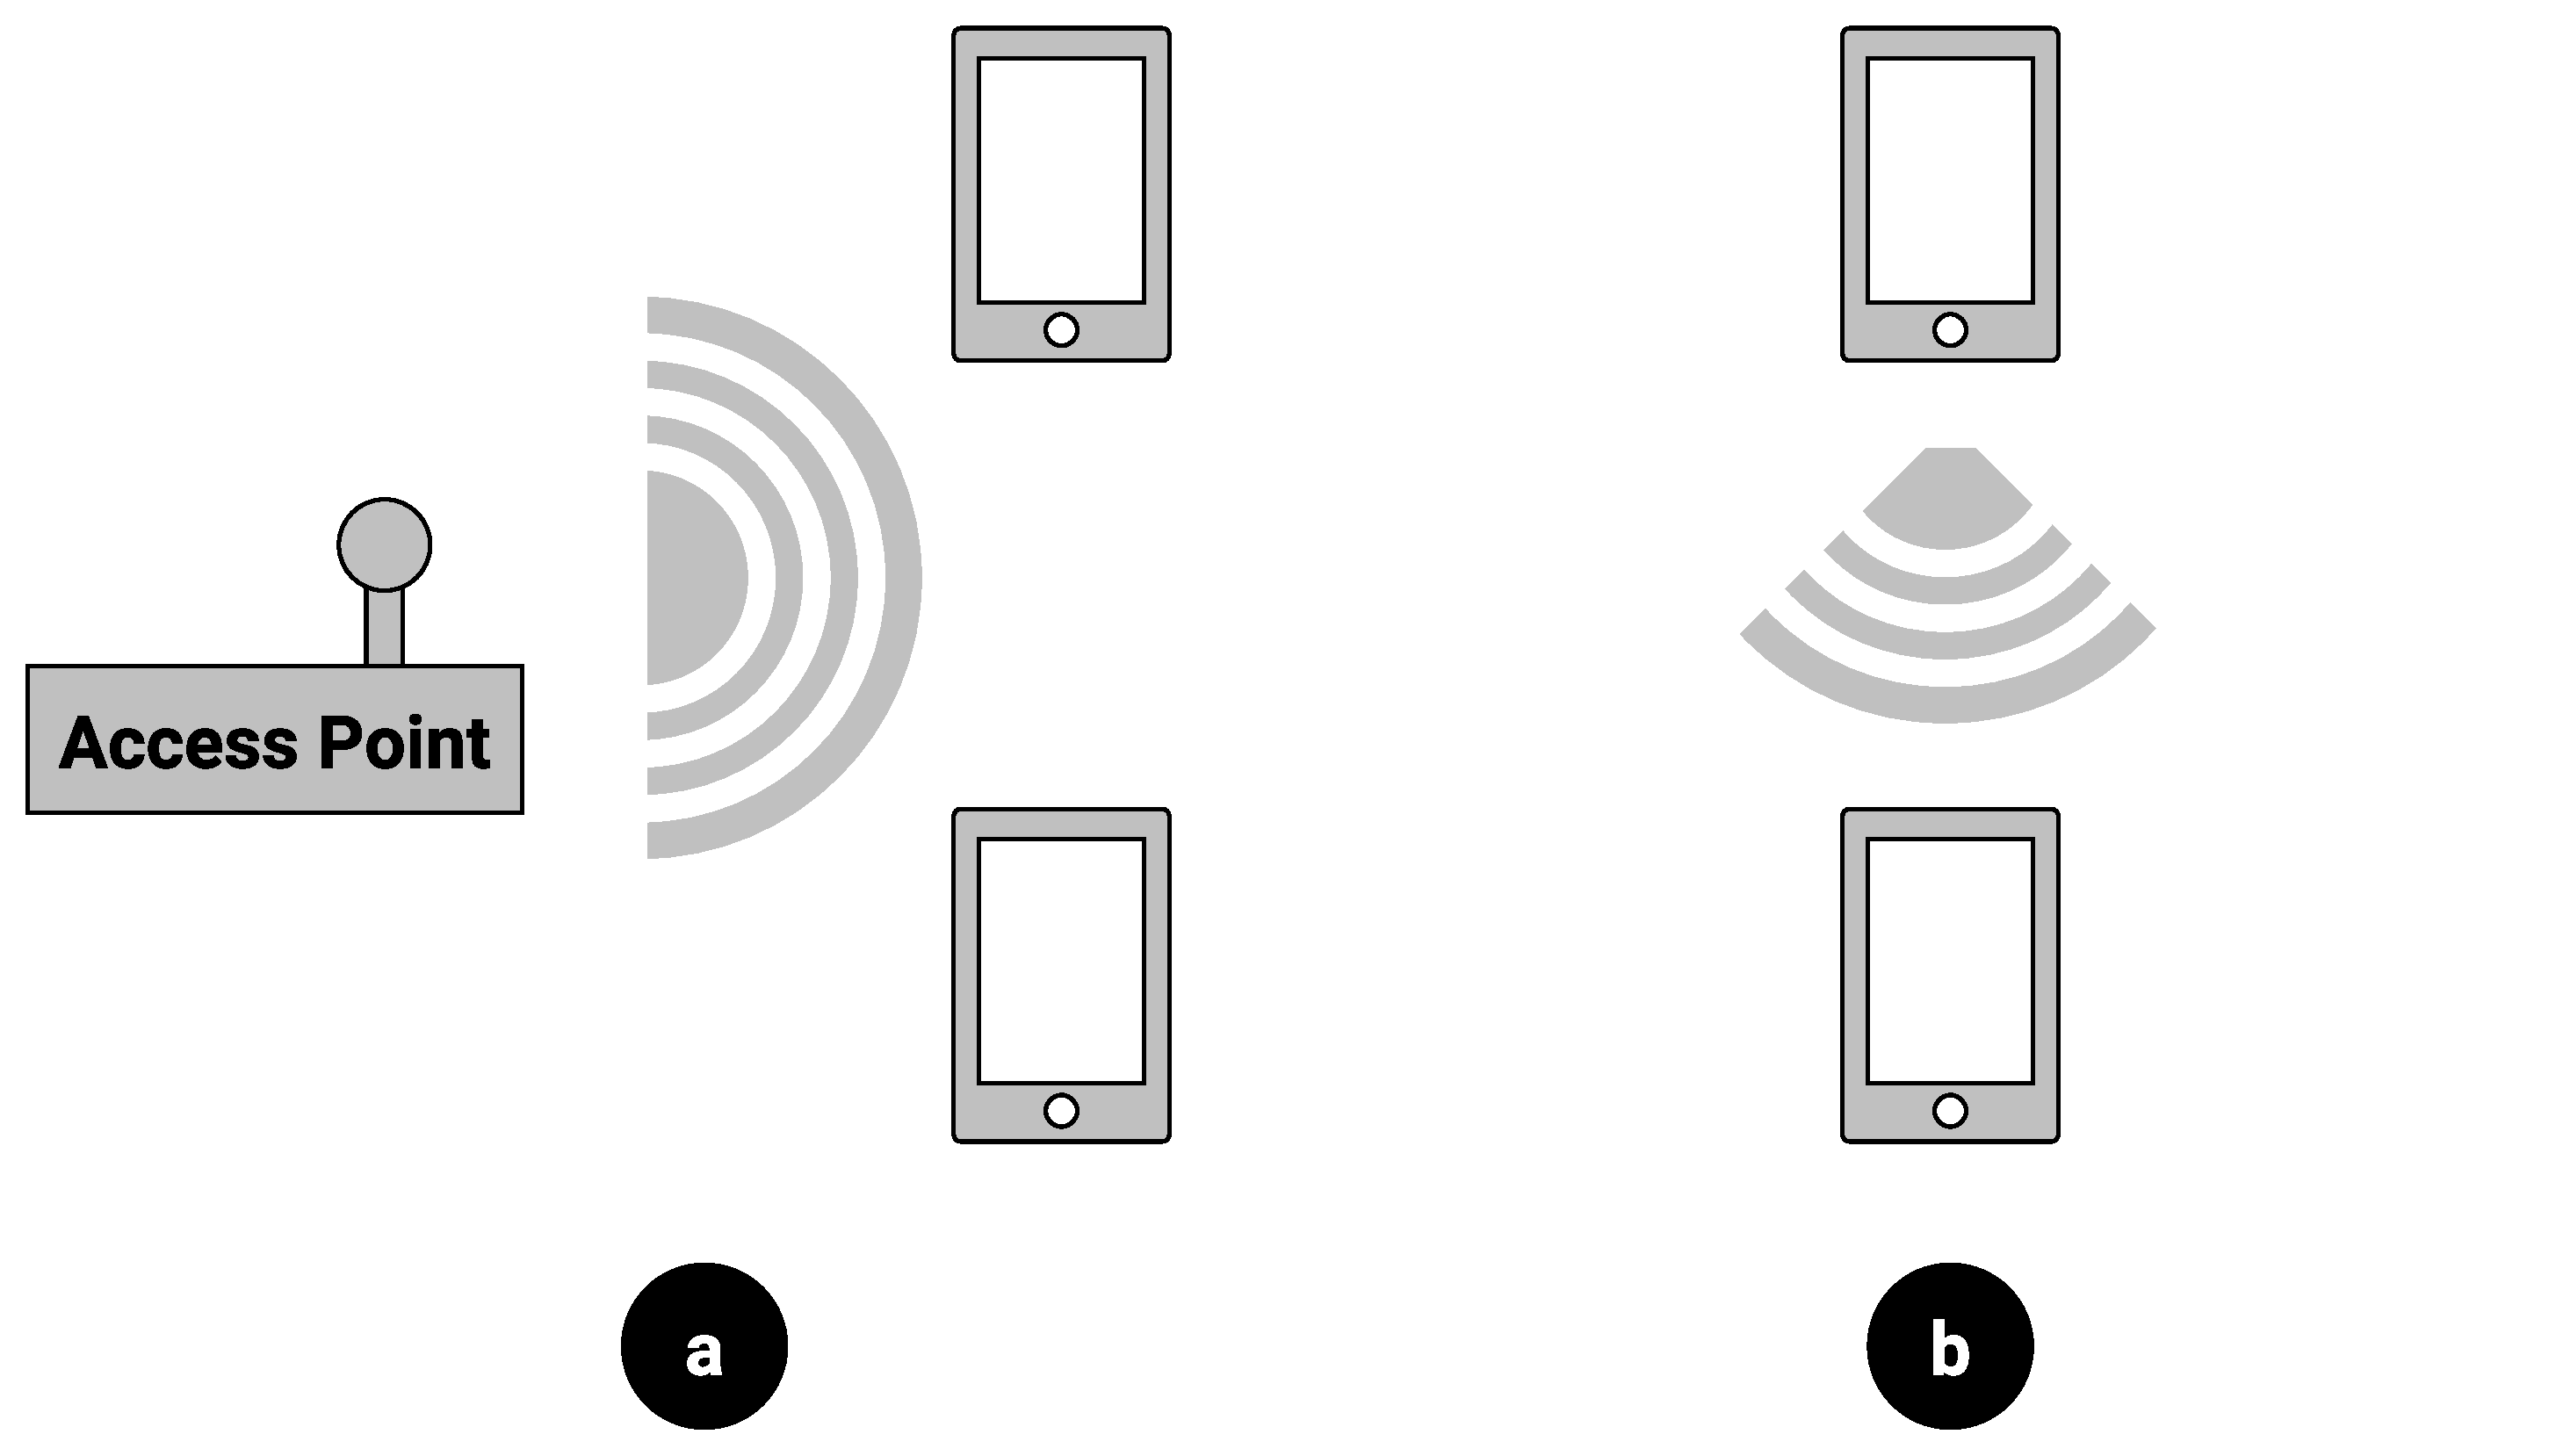
\includegraphics[width=0.7\textwidth]{figures/wifivswifidirect}
	\caption{\label{WiFiVsWiFiDi}Wi-Fi and Wi-Fi Direct network architectures}
\end{figure*}

Before establishing a connection, a device must discover its environment to know if another device is available.
During the discovery process, a device sends regularly a signal that informs about its presence.
The Android Wi-Fi Direct implementation provides the Domain Name System Service Discovery (DNS-SD) protocol that permit to discover other device services that are within range.
This DNS-SD broadcast a set of key/value information that can be read by other devices.
For instance, a broadcast can contain information about the port that will be used to exchange data, the name of the service that is provided, etc.
Devices that are in discovery mode can then filter devices and choose devices that correspond to their connection requirement.
In our implementation, the discovery process is running until the Wi-Fi Direct module is stopped or the Wi-Fi connection is disabled on the device.
\\

After a connection is established between two devices, a private network is created to allow communication through sockets.
The time to establish a connection is about 3 to 5 seconds, but can take up to 2 minutes in the worst cases.
To prevent eventual issues, we set up a timeout to 1 minute per connection.
After this time, device connected or not, the Wi-Fi Direct instance is reset and a new one is instantiated.
The particularity of Wi-Fi Direct communication is that one device on the network is named Group Owner (GO).
The GO is unique for a specific connection and it is the only one that knows all other devices in the private network.
The other connected devices are named Client.
The clients cannot communicate directly with other devices connected to the private network.
They can only communicate with the GO.
\\

This drawback in communication is not embarrassing in our case because we consider that a device can be connected and communicate with only one other device at a time.
In our case, we consider that a device is connected to a single device at a time.
A connection is only made between two devices, no more.
Our implementation does not request for a connection with a device that is already connected with another.
In our implementation, when a connection is successfully processed, each device sends his shared data and add the device to an ephemeral history.
A device is kept in the history an hour to prevent multiple sending of the same data to the same data.
\\

The Wi-Fi Direct implementation requires a user interaction the first time where two devices try to connect each others.
This user's acknowledgement can be seen as a drawback in an opportunistic networking because it cuts the flow of hidden interactions between each device, but this interaction requested only the first time a connection is made between two devices.
If the user accepts the connection request, the following connection with the same device will be automatic and do not ask again for user interaction until the next system reboot or Wi-Fi Direct cleaning groups.
A cleaning function that automatically removes the Wi-Fi Direct groups each time the Wi-Fi Direct is started.
We think that the user acknowledgment is important because it enhances the privacy awareness of the user by informing him that his data will be exchanged with another device.
\\

For more details about this technology, a good study made by Conti et al.~\cite{DBLP:conf/wd/ContiDMP13} present specificity of Wi-Fi Direct connections.

\subsection{Peer Sampling Service}

We provide our dissemination solution as a library that can be used in applications that required a data dissemination layer before sending data to a server.
\\

The architecture of the library is exposed on the Figure~\ref{Fougere}.

\begin{figure*}[h]
	\centering
	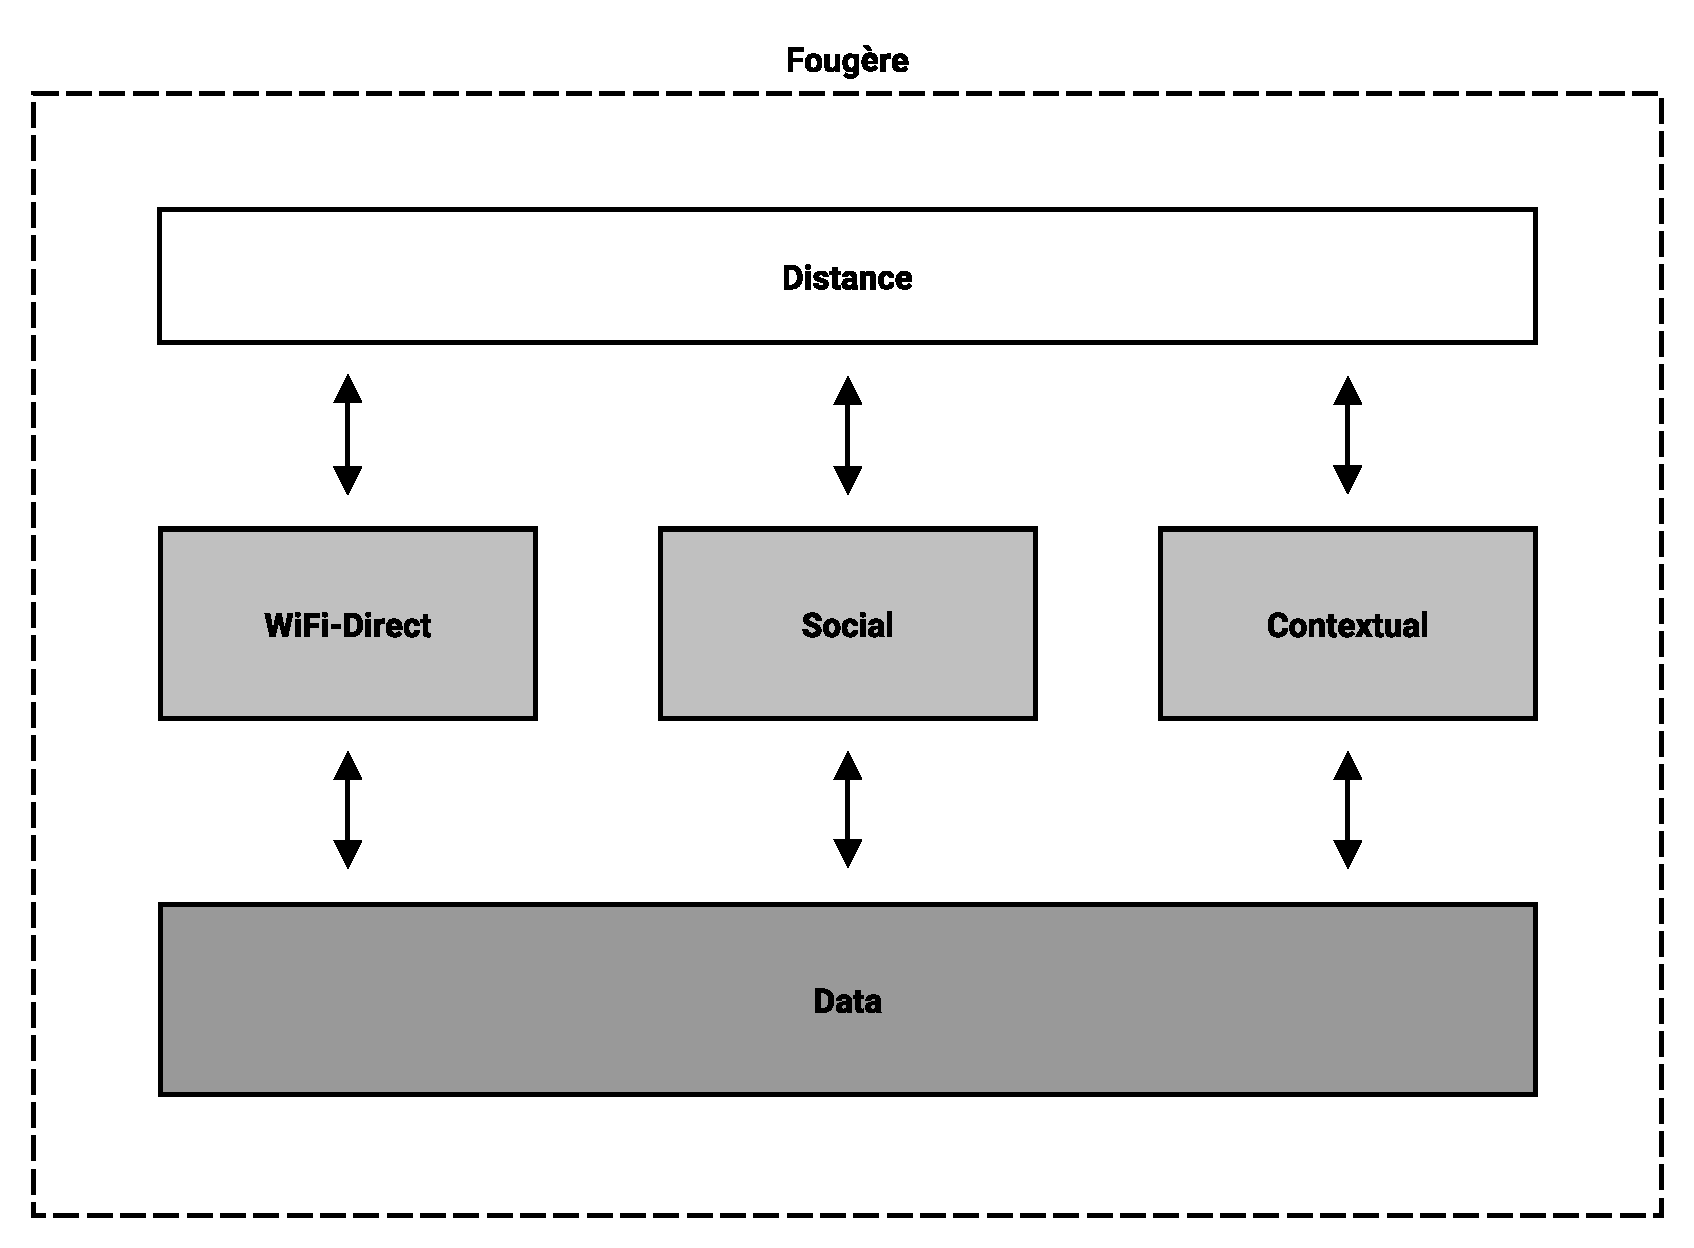
\includegraphics[width=0.7\textwidth]{figures/fougere}
	\caption{\label{Fougere} Foug\`ere architecture}
\end{figure*}

The library includes a database that regroups all data that will be disseminated, 3 default modules that are relative to our proposal: Wi-Fi Direct (Physical), Social and Contextual and a Distance class that takes choices during the dissemination process.
\\

Foug\`ere has a database that contains all data to disseminate.
This is the application implementing Foug\`ere that fill the database by passing it to the Foug\`ere instance.
A data cannot be in multiple module at a time.
\\

The Distance class is linked with each module.
This is the class that is in charge to determine if the data will be sent to the user.
When a module is able to disseminate data, it requests to the Distance class the ability to disseminate.
According to the status of the process, the module sends it to the Distance which update the user distance value.
\\

Each module needs to be able to receive data because in Foug\`ere, the global data are dispatched at a specific time (e.g., each day at midnight) through the enabled modules.
When the dispatch process is started, all data that are in each module are recovered and regrouped in the global database to be re-dispatched.
By this way, we reshuffle the data and allow to disseminate with another method.
For instance, a data can be sent the first time with the Wi-Fi Direct layer and a second time with the Social one.
\\

The Figure~\ref{WiFiDiServInt} illustrates the process of the Physical type dissemination using the Wi-Fi Direct technology.

\begin{figure*}[h]
	\centering
	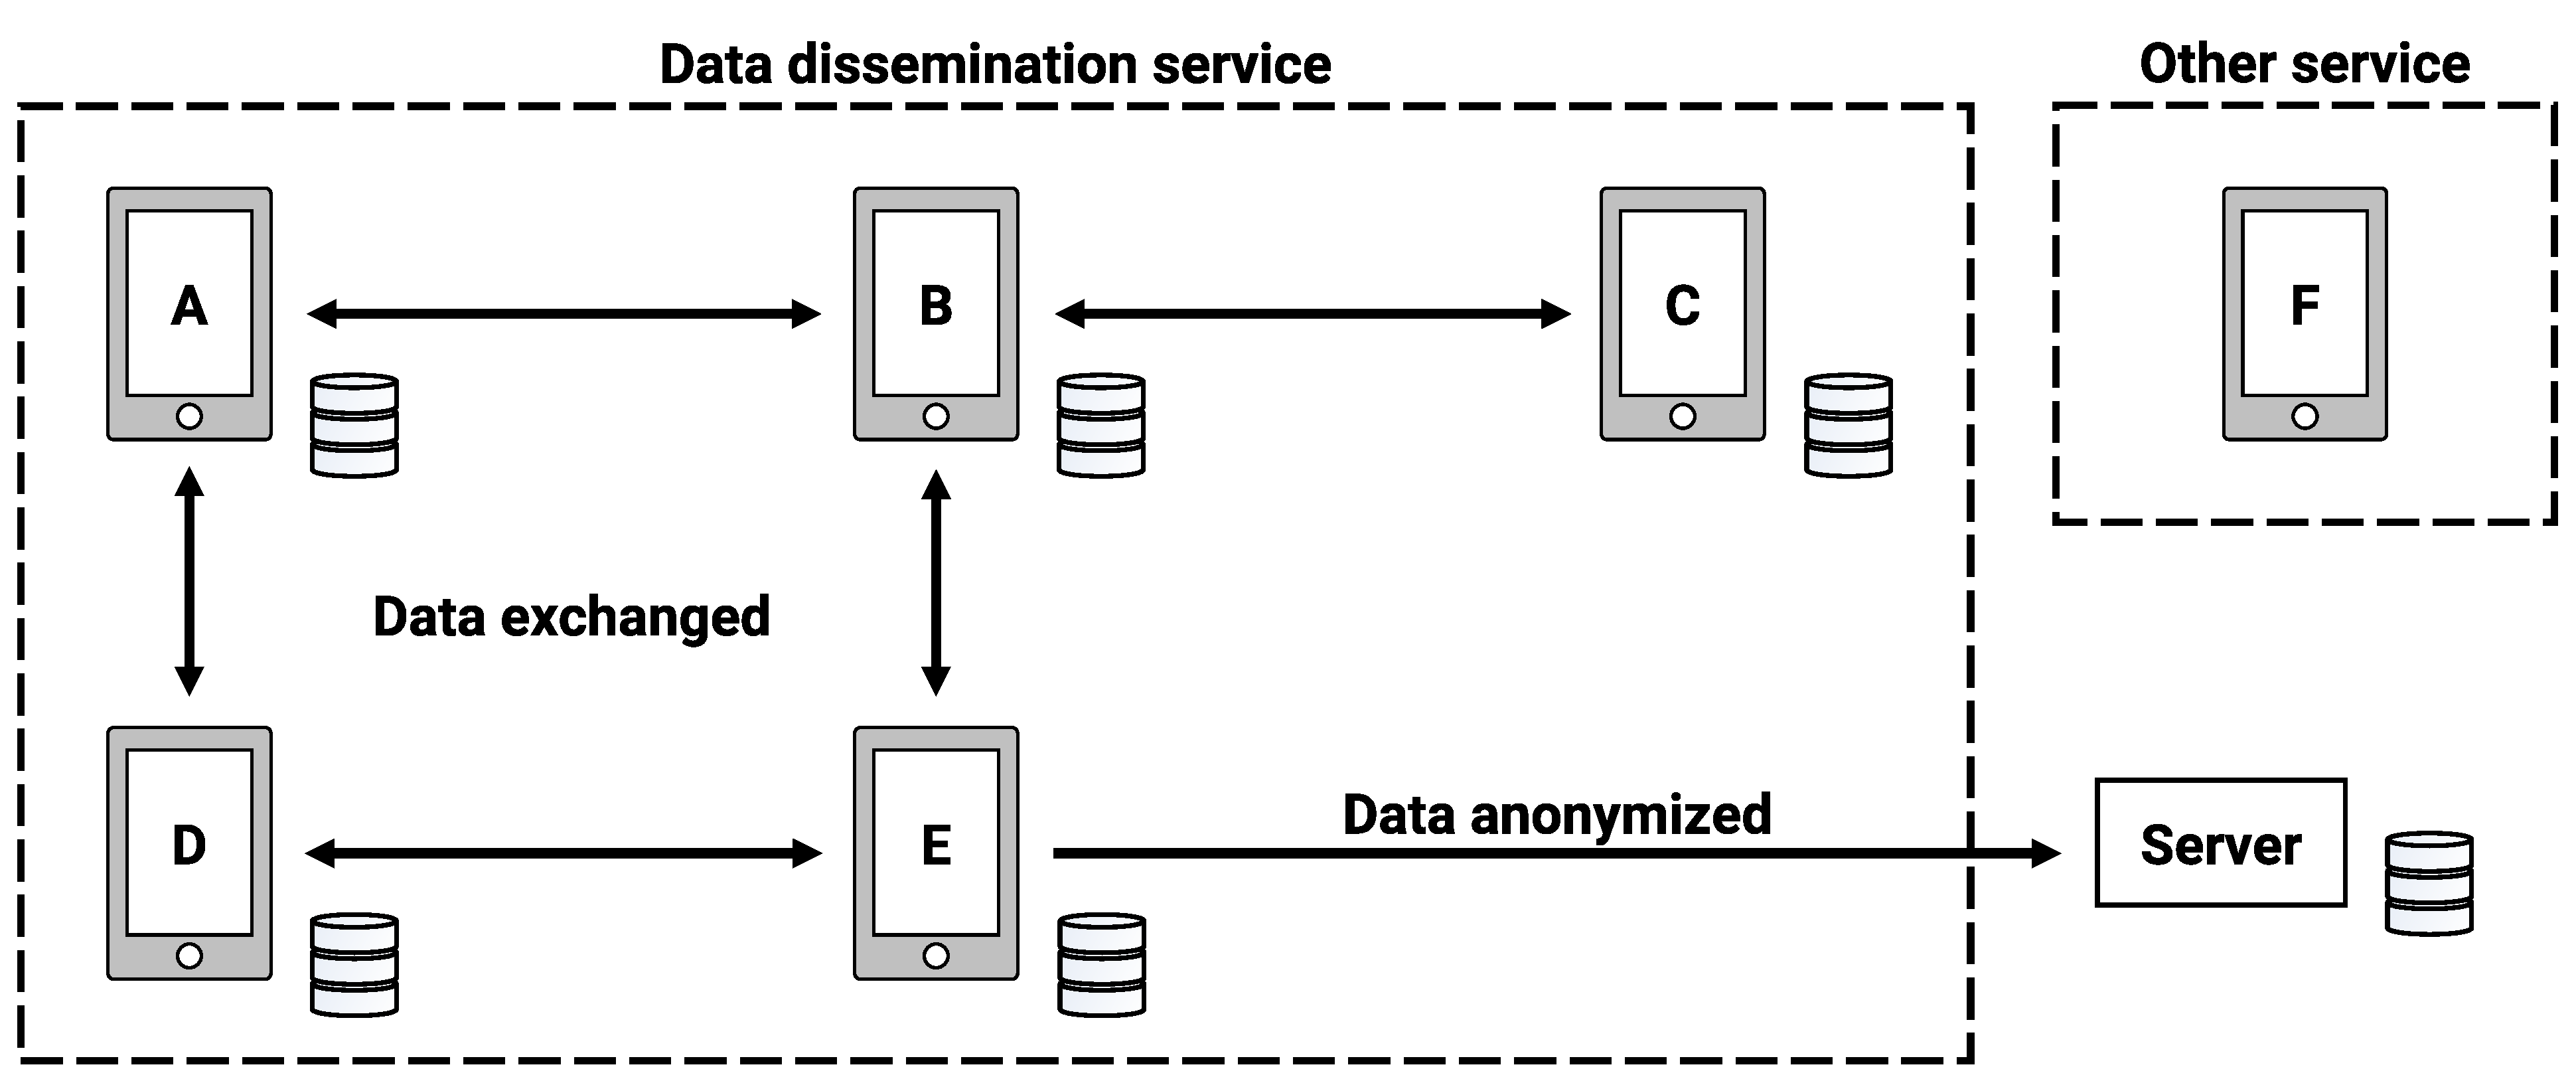
\includegraphics[width=\textwidth]{figures/wifidirect}
	\caption{\label{WiFiDiServInt} Wi-Fi Direct service interactions}
\end{figure*}

As explained above, the Wi-Fi Direct provides a service discovery that allows to provide information during the discovery. 
In this example, the devices A, B, C, D and E provide the data dissemination service where F provides another one.
This indicates that F does not participate in the dissemination and no request will be sent to it by the others.
Where devices are close enough, they can communicate and exchange data.
The data are exchanged and pass through multiple devices.
When the requirements of a data are all reached, the device sends this data to the end-server 

%%%% END OK
	
	\section{Evaluation}
	\label{sec:evaluation}
	
%%%% OK

In this section, we present our own large-scale emulation platform called AndroFleet that provides us a good testing tool for our approach and the evaluation protocol that we will conduct.

Applications developed for the mobile platforms are difficult to test.
When comes the time of the evaluation, 3 ways offers to developers:
\begin{itemize}
    \item testing on real devices
    \item testing on simulators
    \item testing on emulators
\end{itemize}

The first case, testing an application on a real device, is the perfect case because the behaviour of the application is the real one.
However, in the context of crowd of device, this method does not scale and is not practicable and it will really difficult to reproduce users' movement.
It cannot reproduce realistic events that can be encountered in real deployments. 
This method is not the best for a large-scale testing.

The second case is to test the application on simulators.
The simulation platforms are very good when the testing require performance and rapidity of execution, but they do not guarantee that the model simulated is applicable in practice because simulation are just mimicking platforms.
The simulators aim to reproduce the basic--or a subtract--behaviour of a system.

At last, the case that we choose for our platform is the emulation.
The emulators differ from simulations because they aim to exactly replicate the behaviour of a system.
This allows to test the application as near as possible of a real usage.
The drawback of the default emulator proposed by Android is that it does not support proximity wireless interactions.

To sum up, because of a lack of support for Wi-Fi Direct and large-scale deployment of the standard emulator, we choose to develop an emulation platform that is closer to the real behaviour of the system than the simulation.
This emulation platform includes a Wi-Fi Direct simulation layer.
Because we are interested in the data exchange of the data, we do not have a need of exact behaviour for the Wi-Fi Direct.

\subsection{Overview of AndroFleet}

AndroFleet is a large-scale emulation platform that allows to test our Android library.
The platform deploys and runs a large amount of emulators at the same time on a single or multiple hosts.
AndroFleet allows to run GPS location scenarios that reproduced real users' movements.
The experiments are reproducible, which allows to compare different approaches.
Lastly, the platform includes a Wi-Fi Direct simulator that allows the use of the Wi-Fi Direct in the Android emulators.
To be able to use the Wi-Fi Direct simulator, the tested application need to be a little bit refactored by replacing the legacy imports with ours (we propose the exact same class name, only the package name is modified) and, initializing the Wi-Fi Direct manager with our new constructor.

We choose to use the Docker technology because it allows to package and deploy containers easily on different hosts.
Moreover, this technology allows to reproduce behaviours because each time a container is launched, a clean instance of the system is set.
Finally, we use Weave, a technology working with Docker, which manages the containers' network.

\begin{figure*}[h]
    \centering
    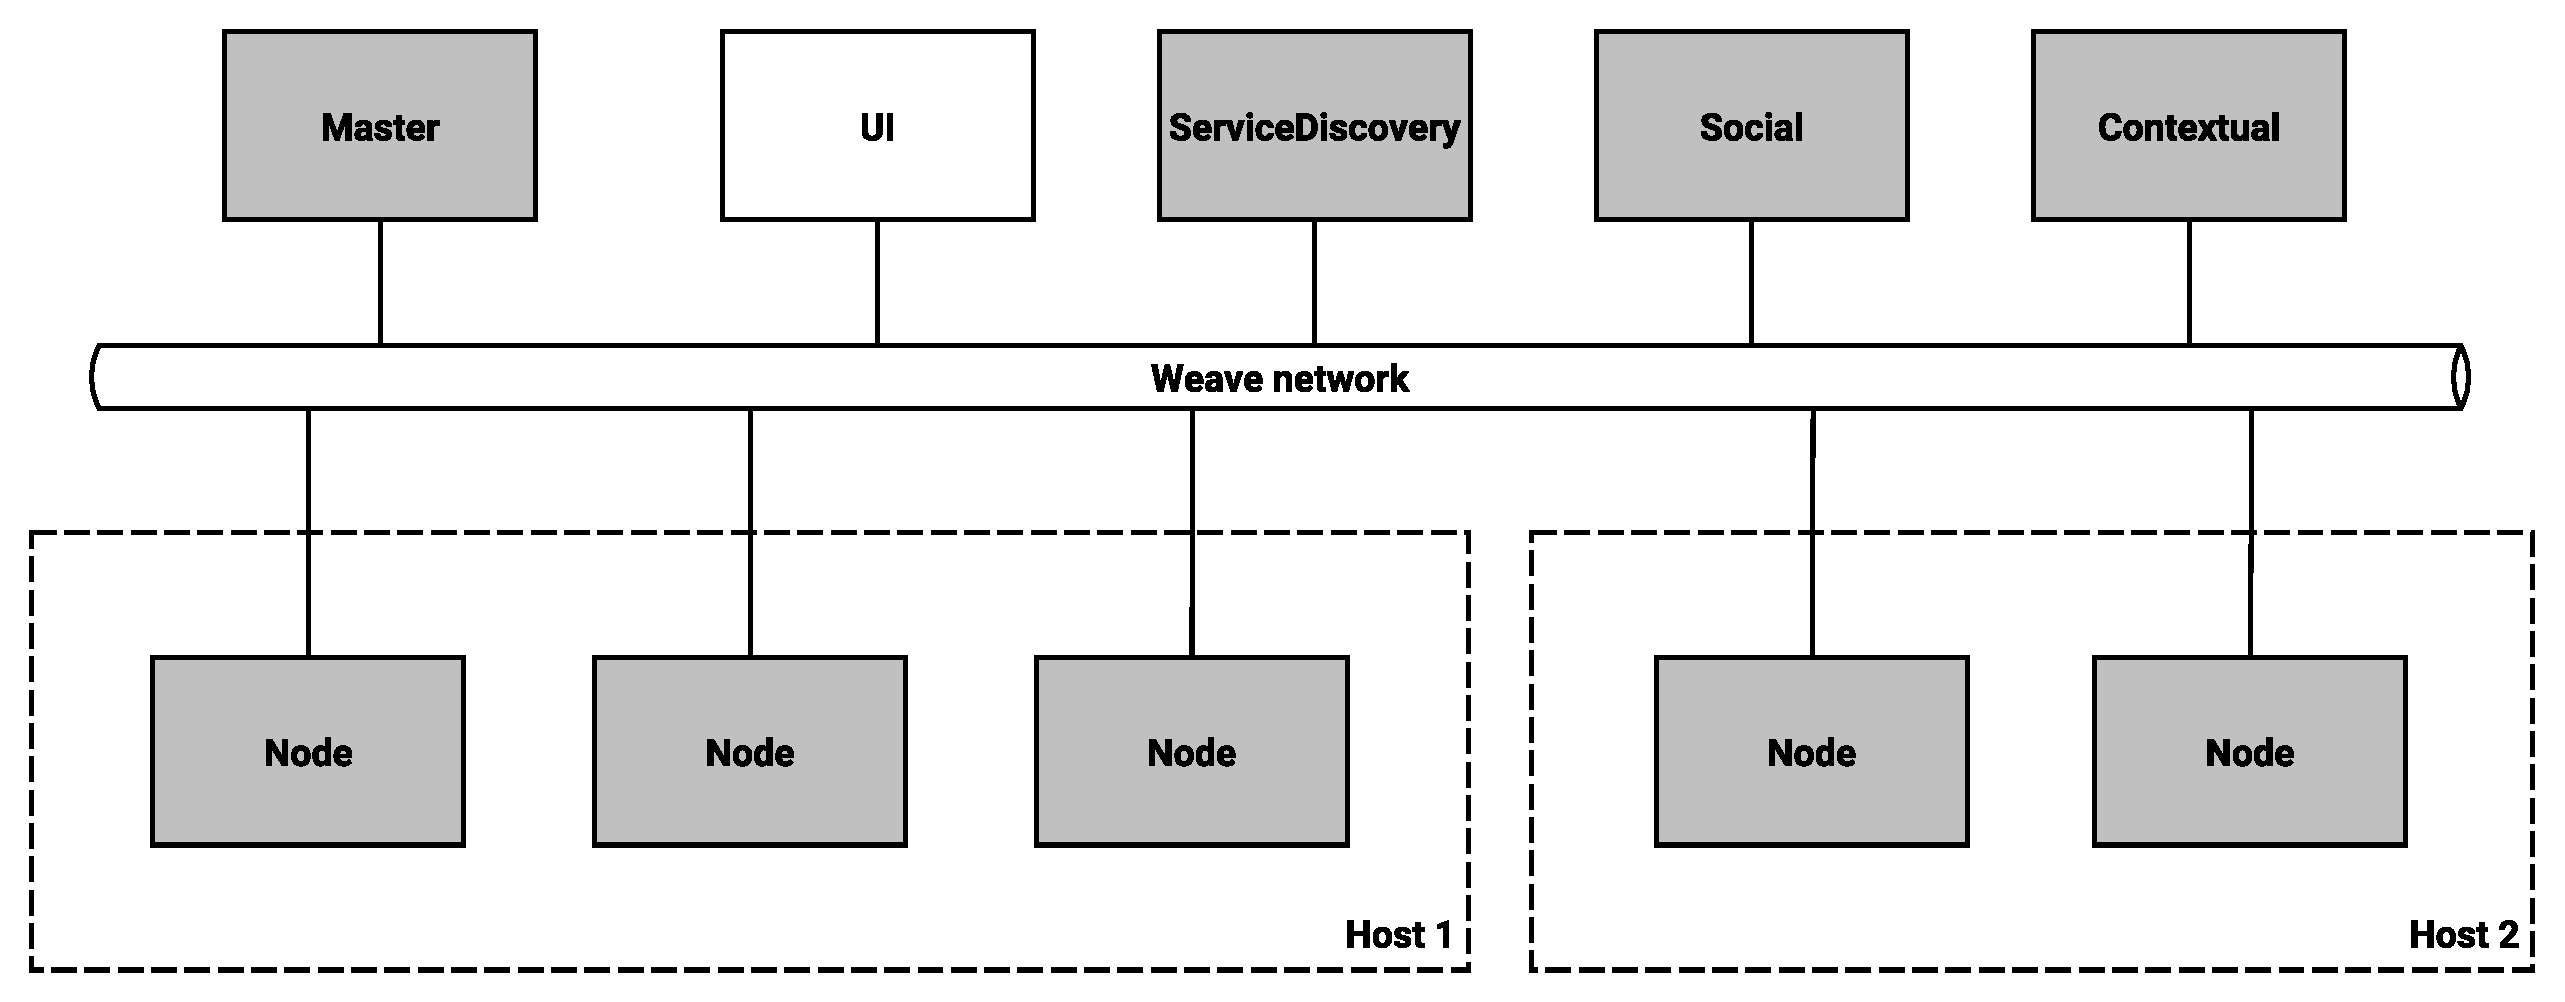
\includegraphics[width=\textwidth]{figures/androfleet}
    \caption{\label{AndroFleet} AndroFleet architecture}
\end{figure*}

The architecture of AndroFleet, presented in the Figure~\ref{AndroFleet}, is composed of 5 elements: Master, Node, ServiceDiscovery, Social, Contextual and UI.
All these elements are packaged and regrouped in a single Docker container.
This container includes an Android emulator that will be run by the Node.

The Master is the main element of the architecture.
It communicates with all other elements of the platform.
For instance, this element is responsible to attribute a scenario to each node container connected.
The Master synchronizes elements of the system.
It allows to control emulation steps with a Command Line Interface and provides information about the progress of the emulation.

The Node element is responsible to launch the Android emulator included in the container and play a GPS scenario.

The ServiceDiscovery element is used for the Wi-Fi Direct simulator.
It allows to the devices to discover themselves.
A Node can request it a list of all its neighbors given its current GPS position.

The Social elements contain information of existing links that exist between emulated users.
The element generates for each running Node its social links.

The Contextual element has the same behaviour as the Social one.
This element generates contextual information for each Node.

The UI is an optional part that can be used to visualize the GPS position of each Android emulator on a map.

A GeoLife parser is included.
It permits to recreate files that are used in our experiment.

\subsection{Evaluation Protocol}

%%%% END OK


We project to evaluate our approach with our AndroFleet platform.




Then, we evaluate the scenarii runner on the well known GeoLife dataset.
We choose Geolife because it is the reference database used by researchers in the geo-location privacy research.
Geolife is a GPS trajectory dataset collected by 178 different users in a period of over 4 years. 
This dataset contains a total of 17,621 trajectories.

Each trace is timestamped.

We process the traces and see if WiFi-Direct can appear with these.

Geolife dataset
We run experiments using the Microsoft’s Geolife
dataset that is a GPS trajectory dataset.
This dataset is made of 182 users for a period of over three years.
In this dataset, a GPS trajectory is represented by a
sequence of time-stamped points.
Each points contains a latitude, longitude and altitude value.
The distance cover by the dataset is about 1.2 million kilometers.
The total duration of timestamp traces is about 48.000 hours.
About 90\% of data logged are spaced under 5 seconds.


so we process Geolife data to regroup traces 

%\subsection{Evaluation Results}
	
	\section{Related Work}
	\label{sec:related_work}
	
%%%% OK

In this section, we discuss the relevant literature about privacy-preserving data dissemination, privacy in Mobile Crowd Sensing (MCS), location-based privacy and related work on mobile devices emulation.

\subsection{Privacy-Preserving Data Dissemination}

Privacy-preserving is a very popular research field.
It exists several research works that propose solutions to enhance the privacy-preserving of users.

The proposal of Lilien et al.~\cite{DBLP:journals/tsmc/LilienB06} use the trust concepts and propose a data self destroy method where the data are automatically degraded when threats are detected.
During a data exchange, the users must trust themselves.
There is always an entity that is weaker than the other when they must prove their identities.
This is called the asymmetric trust relationship.
Trust communications required to trade the privacy to process.
Their approach is a protective one.
They do not try to anonymize the data, but they allow a user to control the dissemination of his data.
Unlike our approach, they do not propose to hide the producer of a data because the producer is known in the meta-data added with the data.
Their technique uses a notion of trusted distance.
Their solution uses a notion of trusted distance.
They use it to degrade the quality of the data when the distance is too weak.
Finally, they do not use their distance notion for the dissemination process like we do.

Another work using the trust relationship concepts is introduced by Singh et al.~\cite{DBLP:conf/icdcs/SinghUSV12}.
They propose a protocol that disseminates data among users that have trust relationships.
They use the users' relationships to construct a new privacy preserving graph to disseminate data. 
We use the principle of the social trust graph to disseminate data between trusted users.

Data disseminated through multiple users can take a lot of time to reach their final goals.
P. Zhong and R.Lu~\cite{DBLP:conf/iccoms/ZhongL14} propose a data dissemination protocol called PAD.
This protocol uses a principle called active user that allows to select the most active users in the system to deliver more efficiently a data.
The proposition uses the Paillier crypto-system to encrypt data that provides a way to add encrypted data to a previous one without knowing it. 
With this process, there are able to group multiple data by keeping it safe.
With this process, there are able to group multiple data by keeping it safe.
They tested their protocol in a simulator but not in a real case.

Another usage for data dissemination protocols is proposed by Boutet et al.~\cite{DBLP:journals/computing/BoutetFGJK16}.
They propose a mechanism of collaborative filter that do not reveal the participants' filter preferences.
Instead of only sending the data to other participants, a data dissemination protocol can filter the data--according to the predefined participant rules--that pass through the different participants.
Their mechanism is capable to automatically drop the data that could leak a bit too much information about a user.

Lu et al.~\cite{DBLP:conf/infocom/LuLSCS13} propose a scheme for opportunistic network called Incentive and Privacy-Aware data Dissemination (IPAD).
Their solution uses a social layer that permits the dissemination through trusted nodes.
We use their social notion in our solution by permitting a dissemination through a possible trusted set of other participants.

For some applications, the response time is important (e.g. in localized based services).
Private Pooling, the collaborative sensing protocol proposed by Wiesner et al.~\cite{DBLP:conf/mobisec/WiesnerDD11} focuses on decoupling the data from its producers.
Their protocol reaches to break the linkability of the data to a specific user.
They do not discuss possible advantages of using proximity technology like Bluetooth or WiFi-Direct.
Their approach requires a network connection to work.
Unlike our approach, their case of study required a very short responds time.
Their requirement is not important for us because, in a case where the data are Geo-located, introducing a delay in the exchange can be better in a privacy-preserving view.

In the cases where the data transmission delay is not important, the users of the system can exchange and store temporarily the data received by the others before resend it later.
Guo et al.~\cite{DBLP:conf/infocom/GuoZYF13} propose a dissemination scheme for delay tolerant networks that is based on users similarities via attributes like position, language, country, etc.
In their scheme, a user shares his data with others only where their profiles are close enough to his own profile.
Unlike our evaluation, they consider that all users are always close enough to communicate that is not always the case--by far--in reality.

Finally, the gossip-based protocols are very popular in applications that contain a large number of participants because of the reliability and the scalability of these types of protocols.
A generic framework proposed by Jelasity et al.~\cite{DBLP:conf/middleware/JelasityGKS04} permits to create peer sampling services based on gossip communication protocols.
They compare the convergence and the randomness of different gossip based approaches and conclude that gossip-base protocols are reliable and scalable.

\subsection{Privacy in MCS}

Many applications in participatory sensing systems are not used because of privacy concerns. 
The main challenge is to apply privacy-preserving method without losing the quality of the data.

In this field, Vergara-Laurens et al.~\cite{DBLP:conf/percom/Vergara-LaurensML14} propose a privacy-preserving mechanism to anonymize data without losing the data quality.
Their approach is focused on Geo-located data and is not decentralized
They work on Point Of Interest of data (e.g., the user home place, his workplace, etc.).
Each time a data is reported by a user, a proxy server recalculates a new fuzzy Point Of Interest according to the data value that is reported.

Boutsis and Kalogeraki~\cite{DBLP:conf/percom/BoutsisK13} introduce a participatory sensing middleware for the Android platform that preserve users' privacy (in particular for the location data).
Unlike current centralized solutions like the APISENSE platform, their solution is decentralized.
Like our approach, their proposal maintains the privacy on the user side before sending the data to the server.
Their work is based on misco, a MapReduce system for mobile devices.
Their tool does not take interest of proximity exchange technologies like Bluetooth or Wi-Fi Direct, it uses Wi-Fi and 3G networks to exchange data.

The users may not want to contribute due to possible privacy leakage and lack of incentives.
To fix this issue, Li and Cao~\cite{DBLP:conf/percom/LiC13} propose a participatory reward system for the collaborative mobile sensing systems.
They provide a scheme where the users earn credits when they contribute to the system.
Earn credits can be converted to real money or invested in data collects.
Their scheme rewards and protects users that contribute to the system.
Their solution is implemented in 2 ways: one using a trusted third party server and the second without.

At last, Groat et al.~\cite{DBLP:conf/percom/GroatEHHF12} present a scheme for participatory sensing that preserves users' privacy for multidimensional data by using negative surveys.
Their method perturbs the data which hide the real user location.
The proposal allows to not encrypt data before sending it, which permits a gain in term of data transmition cost.
Their approach allows to customize privacy and accuracy.
Their proposal is useful in the case of data accuracy can be degraded.

\subsection{Location-Based Privacy}

Geo-located data expose the users to substantial privacy threat.
Those data reveal a lot of information about the users like health information, path habits, etc.
The identity of a user can be determined even if the location data are sanitized.
In the field of location-base privacy, general approaches implied central servers that know everybody's locations.

An overview of attack scenarios, data transformations and privacy guarantees on location data is introduced by Terrovitis~\cite{DBLP:journals/sigkdd/Terrovitis11}.
The author reminds the existing k-anonymity and l-diversity methods that allow to hide users and prevent against linkage.
These methods are largely used, but are on the server side of the platforms.
A predominant technique used third party servers that provide alternative locations instead of real users locations.
This solution includes trusted servers that work as proxy to hide real users' locations.
The solutions where the servers can't be trusted required obfuscation methods on the user side.
For instance, a user can send multiple locations to servers to hide his real position
There are 2 scenarios arising in the case where the users are allowed to communicate with each other.
The first is where a user does not trust the server, nor the other users.
The second is where the users trust each other but do not trust the end-server--this is typically study case.
In this second case, the techniques are generally based on spatial cloaking that generalize a location to a specific and generic area.
The splitting of the real locations with others is another method that is used.
Other techniques use dummy locations where the real user location is a subset of the location area requested to the server.
For the data transformation and protection methods, a trade-off need to be found between data accuracy and privacy.
Location data are generally associated with timestamps, which is leaking a lot of information that can be computed.
The author shows that systems that do not use anonymization techniques are close to use equivalence classes or spatial cloaking techniques.

The proposal of Werner~\cite{DBLP:conf/mobisec/Werner10} is a method to protect the users' privacy in location based services.
The author proposes an approach to exchange location data.
His first example is where 2 users that want to know where are each other and receive a notification where there are close.
Werner made it by sending encrypted data--using an asymmetric encryption--to a server with an identifier that correspond to a user.
This method required that the sender knows the public key of the receiver to encrypt the data.  
The users can exchange public keys via SMS or QRCode before which does not required a server to deliver these keys.
Only the receiver can decrypt the data and show the location of the sender.
Werner proposes another example where a company wants to offer promotions.
His solution is to generalize the user location to a larger area and recover all services in the area.
Then, the user receives all available services that can be filtered to get only the services that are close to him.

Finally, where k-anonymity methods are generally realized on the server side, Zhong and Hengartner~\cite{DBLP:conf/percom/ZhongH09} propose a distributed k-anonymity for location based systems that needs neither a single trusted server nor users to trust each other.
Their method can be applied on current used architectures and assume multiple servers.
The servers can be controlled by external organizations that split knowledge of users' locations where each server knows only a few parts of all users' locations of the system.
In their proposal, the users' requests pass through location brokers that hide the real location of the users.

\subsection{Mobile Devices Emulation}

The number of emulation tools allowing proximity interactions through Wi-Fi Direct is poor.
Generally, studies are validated on network simulators that are good, but are not close of a real use of an application.

Wehrle et al.~\cite{DBLP:conf/simutools/WeingartnerLW11} introduce a network emulation architecture that focuses on network interactions.
Their focus is on wireless communication software.
They use the ns-3 tool to simulate network transmissions.
They provide an Android plug-in that uses an old version of the Android emulator.
Our focus is more on the general behaviour of data dissemination instead of the exact propagation and exchange through the network--which can be monitored with ns-3.

Bruno et al.~\cite{DBLP:journals/amsys/Bruno0F15} propose a solution that emulates Wi-Fi Direct for the Android platform.
Their emulation solution is focused on Wi-Fi Direct communications and aims to facilitate the testing of applications.
The platform is scalable because it can be deployed on a cloud infrastructure.
Like our emulation platform, the tested application code must be refactored a little bit to import and initialize the Wi-Fi Direct layer.
The drawbacks of their proposal are where we want to control the emulation, we need to pass through a command line interface that is not convenient and, be able to play humans' mobility scenarios is impossible.

At last, Hetu et al.~\cite{DBLP:conf/vtc/HetuHP14} present a simulator that includes traffic, network simulators and a cluster of Android emulators to test Android applications.
Like our proposal, their solution requires code refactoring to work.
Unfortunately, they do not provide the source code of their work that could be very interesting for the crowd-sensing community to share.

%%%% END OK

	
	\section{Conclusion \& Perspectives}
	\label{sec:conclusion_perspectives}
	
%%%% OK

In this report, we presented a data dissemination approach that disseminates data through users of a crowd-sensing platform.
This approach is based on a notion of proximity between users exchange data--proximity that could be Physical, Social or Contextual.
We provide an Android library called Foug\`ere that includes all the concepts presented in this report. 
In addition, we provide a large-scale emulation platform called AndroFleet, which is useful to test--as near as possible of a real usage--Android applications in the context of crowd-sensing.

% Fougère and AndroFleet perspectives

As perspectives, different threat models could be tested on applications using Foug\`ere to see in which cases our approach is efficient and improve it in the cases where it fails.
Foug\`ere could take concern of what type of data is sent and auto adapt the parameters (e.g., the TTL value) in function of the data flow monitored.
The Wi-Fi Direct could implement a new method base on decentralized k-anonymity where a data would be sent to the server only if k instances of this data have been received.
Finally, we could include Foug\`ere in the APISENSE Android application to test his viability in the real world.

Concerning AndroFleet emulator, it could be improved to cover a larger experimentation cases.
We could enrich the implementation of the Wi-Fi Direct simulator for a better and larger support of the technology.
Additionally, the Bluetooth technology could be simulated to offer more a proximity networking alternative.
At last, localized Wi-Fi hotspot could be useful for some experimentations.

% Evaluation perspectives

Future work to become is to run the evaluation protocol described in this report and interpret the results.
Foug\`ere library and AndroFleet are functional and to be able to conduct the results, the only requirement is to well configured each part and run it on the testing server.

Last, but not least, this work will be submitted--at the end of the month of September--to the famous IEEE PerCom conference. 

%%%% END OK

	
	\bibliographystyle{abbrv}
	\bibliography{sommerard-internship}

\end{document}